%% LaTeX2e class for student theses
%% sections/evaluation.tex
%% 
%% Karlsruhe Institute of Technology
%% Institute for Program Structures and Data Organization
%% Chair for Software Design and Quality (SDQ)
%%
%% Dr.-Ing. Erik Burger
%% burger@kit.edu
%%
%% Version 1.3.2, 2017-08-

\chapter{Evaluation}
\label{ch:eval}
After we evaluated the created case study in \autoref{ch:cocome} and \autoref{ch:casestudysystem}, in this chapter the procedure (\autoref{ch:method}) and the used modeling language (PCM \cite{PCM}) are evaluated. The evaluation are also based on a GQM-plan \autoref{GQM_Expl}. The plan for the whole evaluation can be seen in \autoref{GQMPlan}. \\ First, we conduct the evaluation for the applicability of the presente dprocedure, then the expressibility of the modleing language. Afterwards, we summarize the results for the created case study. To conclude the chapter, we discuss the \textit{threats to validity} (\cite{TtoV}).

\begin{figure}
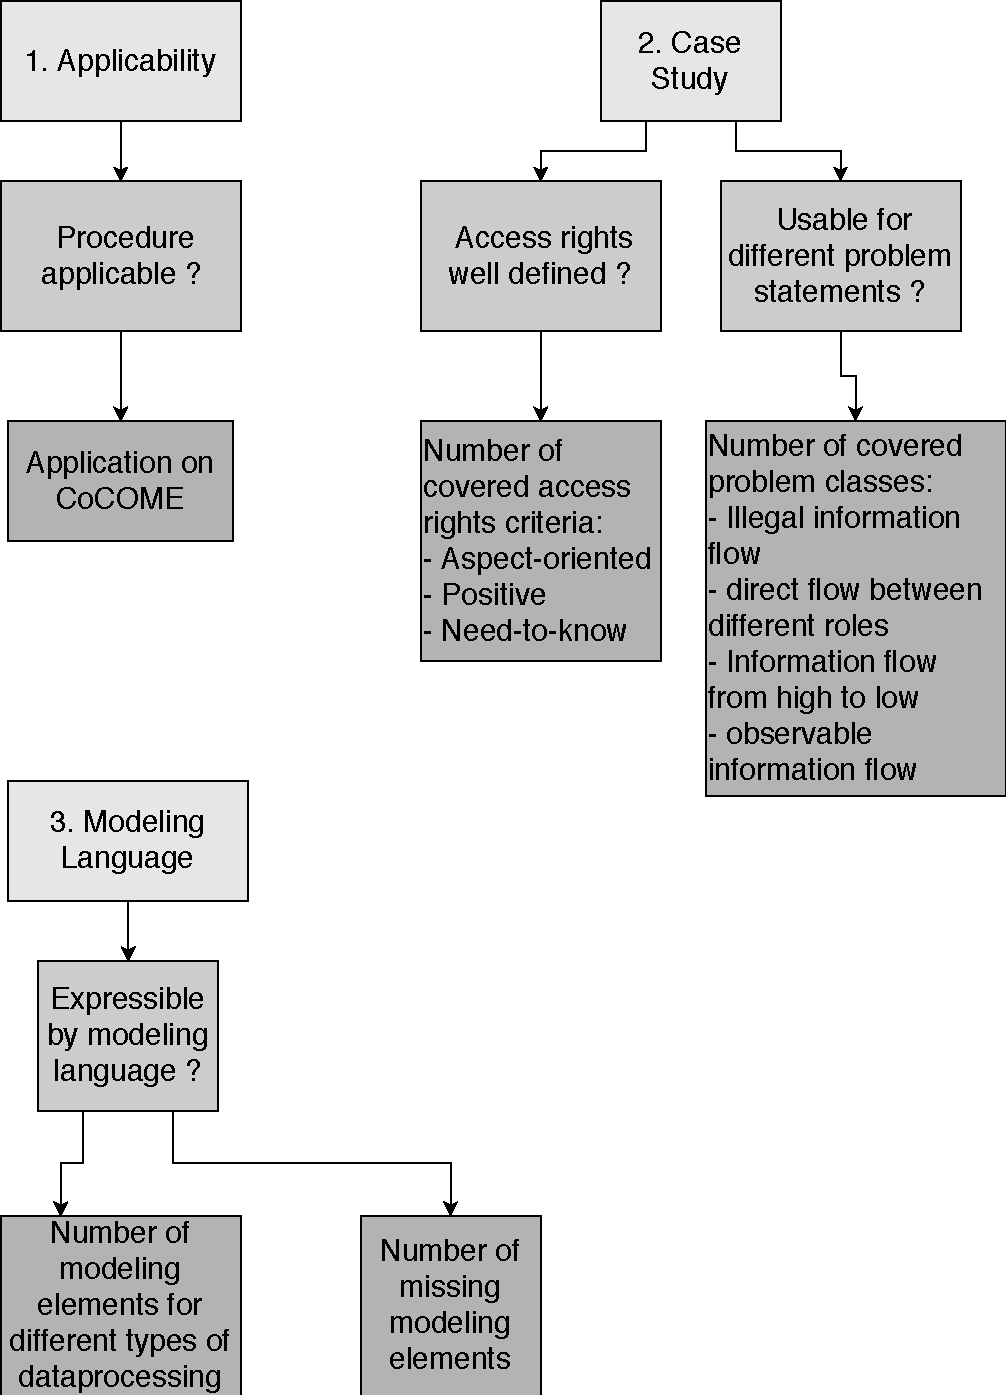
\includegraphics[scale=.8, origin=c ]{logos/OverviewEval.pdf}
\caption{The GQM plan for the three parts of the evaluation. Each part is divided into }
\label{GQMPlan}
\end{figure}

\section{Goal: Applicability of the introduced procedure}
The first aspect we are evaluating is the applicability of the introduced procedure to create case studies from software systems. We evaluate the applicability to verify if its possible to create case studies that later may be used to evaluate approaches for a data-based privacy analysis. The examination if the quality of the created study is sufficient is a separate part and has to be done on a case-by-case basis.  
\subsection{Question: Is the introduced method applicable to an actual system?}
To verify if the goal is achieved, we check if the introduced procedure is applicable to a software system that abstracts the selling process and warehousing of a supermarket group. The metric to answer the question is a successful application to an actual system.  
\subsubsection{Application to the CoCoME system}
The system we chose to apply the method on is CoCoME. We applied the procedure not the whole CoCoME system but only to an excerpt of it. The application to the excerpt and resulting case studies is conducted in \autoref{ch:cocome} and \autoref{ch:casestudysystem}.\\ We successfully applied the procedure to an actual system and created a case study. Therefore, we conclude that the procedure is applicable.
%\section{Usability of the created case study for data-based privacy analysis}
%\label{usage_DBPA}
%The next aspect we evaluated the usability of the created case study. A case study is not useful if it does not meet criteria. The criteria ensure that the case study is in a state where it can be used for data-based data privacy analysis. To ensure this, we evaluate two different parts of the case study. First, we evaluate the defined access rights, then the defined data flows. 


\section{Goal: Expressiveness of data-centric PCM}
In this part, we evaluate the modeling language that is used for the case study. To model the case study, technically speaking, it have to be possible to add two extensions to the system model. First the data flows and ,Secondly ,the defined ACM.\\ We chose to use data-centric PCM as the modeling language % ref auf foundations
By default it is not possible with data-centric PCM to extend models by data flows and an ACM. Therefore we went for the meta-model extension for data-centric PCM from Seifermann \cite{MMextension}. So, this part of the evaluation will mainly focus on the meta model extension for data-centric PCM. 

\subsection{Is the created case study expressible with data-centric PCM ?}
To verify, if the case study is expressible with data-centric PCM, we ar eusijgn two metrics. First we measure which elements are available and then which elements are missing.
\subsubsection{Number of available elements to model the different types of data processing}
The main focus is to verify, if the created case study is expressible with data-centric PCM. We check if it is possible to model all defined operations in the OpM. %ref OpM !!! 
This is also done in a checklist manner.
We defined four operations for the case study in the OpM: transmission of data, alternation of data, operations for relational algebra and operations to model user interaction. 

\paragraph{Transmission data}
This operation describes if components transmit data. An operation for this available in the meta model extension.

\paragraph{Alternation of data}
This is a larger type of operations. All in all, this type describes the alternation of data. This includes
creation of data, merging many points in, for example, into list or set, the splitting of data, like lists, in the single data, etc. With the alternation of data it can happen that the class of data is changed and thus the applying access rights change. To describe the change of the applying access rights an operation is available in the meta model extension. 

\paragraph{Operations relational algebra}
This type of data processing describes the manipulation of database or data requested from databases. The operations for this are available in the meta model extension. 

\paragraph{I/O- operations}
Operations to model the user interactions are also available.

\subsubsection{Number of missing elements for the different }
Currently it is not possible to store the ACM in the same system model. It is possible to define access rights for each data in each component for each role. First, for each data a new access right has to be defined and , secondly, it is not or only with disproportionate effort possible to swap out the access rights or generating the ACM form the model. For the fact, we created our case study \textit{aspect-oriented} (see \cite{}) the current modeling contradicts the concept. Therefore, a model element for the ACM is missing.
\subsubsection{Summary: expressiveness of data-centric PCM}
Now that the two metrics have been collected, we summarize them. The summary of the both metrics is shown in \autoref{PCM_eval_sum}. As it is shown, the only flaw is that the ACM cannot be included in the system model. 
\begin{table}
\begin{tabular}{|c|c|}
\hline 
Meta model  & possible ? \\ 
\hline 
relational algebra & \cmark \\ 
\hline 
I/O operations & \cmark \\ 
\hline 
Transmission of data & \cmark \\ 
\hline 
Change of access rights & \cmark \\ 
\hline 
Alternation of data & \cmark \\ 
\hline 
ACM in system model & \xmark \\
\hline
\end{tabular} 
\caption{Summary for the evaluation for the modeling language.}
\label{PCM_eval_sum}
\end{table}
\section{Evaluation of the created case study}
The evaluation of the created case study is split into two parts: the quality of the access rights and the covered information flow classes. Each part is already conducted in % ref und ref
Here we shortly summarize the results of the single evaluations.
\subsection{Access rights}
Further details on this evaluation can be seen in % ref
Evered and Bögeholz \cite{CaseStudyAndAccessrigths}%
defined seven criteria to review the quality of defined access rights. All in all, the criteria can be divided in three categories: Specification, Comprehensibility and Implementation. \\
\textit{Specification} criteria review the definition of the access rights. \textit{Comprehensibility} criteria mainly reviews the notation and ho clear each is defined. \textit{Implementation} criteria reviews the embedding of the access rights in the implementation.\\
The result of the evaluation are displayed in \autoref{AR_EVAL_SUM2}.
\begin{table}
\begin{tabular}{|c|c|c|}
\hline 
\multicolumn{2}{|c|}{Access rights} & fulfilled? \\ 
\hline 
Specification & Aspect-oriented & \cmark
 \\ 
\hline 
 & Positive & \cmark 
 \\ 
\hline 
 & Need-to-know & \cmark 
 \\ 
\hline 
Comprehensibility & Clear & ? \\ 
\hline 
 & Concise & ? \\ 
\hline 
Implementation & Fundamental & n/a \\ 
\hline 
 & Efficient & n/a \\ 
\hline 
\end{tabular} 
\caption{Summary for the evaluation of the defined access rights.} 
\label{AR_EVAL_SUM2}
\end{table}  

\subsection{Covered information flow classes}
Further details on this evaluation can be seen in \autoref{Eval_infoFlowClasses2}.
In the evaluation we examine which different information flows are covered by the created case study and may later be checked in a data-based privacy analysis. To define different information flow classes, we relied the problem statement \textit{Non-influence} \cite{Noninfluence}. This problem statement includes four different information flow classes: illegal information flow, information flow from high to low, direct information flow between roles and observable information flow. The summary of the covered information flow classes is displayed in 

\begin{table}
\centering
\begin{tabular}{|c|c|} 
\hline 
Data flow & fulfilled? \\ 
\hline 
Illegal information flow & \cmark \\ 
\hline 
Information flow from high to low & \cmark \\  
\hline 
Direct information flow between roles & \xmark \\ 
\hline 
No observable information  flow & \xmark \\
\hline 
\end{tabular}
\caption{Summary for the evaluation of the covered information flow classes of the case study.}
\label{Eval_infoFlowClasses2}
\end{table}

\subsection{Summary for the evaluation of the case study}
We achieved to cover three out of seven criteria (~43\%) for good access right. The evaluation of the criteria in the \textit{Comprehensibilty} class would have exceeded the scope of the thesis. So we cannot make a qualified statement for these criteria. The criteria associated with \textit{Implementaation} class may be omitted in a purely conceptual case study. For instance, this may happen when a complete system is modeled but not implemented yet. We achieved all of the \textit{Specification} criteria with our defined access rights.\\ All in all, we say the number of applicable criteria are dependent on the goal for that the specific case study is created. \newline
We also achieved to cover 50\% of the information flow classes. We coul not achieve to cover all classes due to time constraints of the thesis and therefore missing scenarios.


\section{Threats to validity}

In this section we discuss possible threats to the validity of the evaluation. The general description for this threats are published by Runeson and Höst \cite{CaseStudySoftware} %hie rmal von HEinrich klauen, eventuell
The possible threats are divided into four categories: internal validity, external validity, construct validity and conclusion validity.
\paragraph{Internal validity}
Internal validity describes if the evaluation supports the conclusion. 
\paragraph{External validity}
External validity describes that the results can be generalized.
\paragraph{Construct validity}
Construct validity describes that the measurements for the construct under investigation are correct. In particular, this means that the measurement is not influenced by other factors.
\paragraph{Conclusion validity}
Conclusion validity describes that evaluation is based on \textit{reasonable} data, for instance statistical data, to minimize or eliminate the subjective view of the researcher.
\subsection{Analysis of the evaluation}
We analyze the three parts for the evaluation carried out and identified aspects that could pose a threat to the validity of the results. The aspects are: the procedure, the defined access rights and the covered information flow classes. In \autoref{TtoV_sum} a categorization for the aspects is shown.
\paragraph{I: Procedure}
The introduced procedure has only been applied to an excerpt of a system. This endangers the \textit{external validity}. The procedure works for CoCoME but this cannot be ensured in general.
\paragraph{II: Access rights}
Three out of seven criteria were evaluated for different reasons. This could be a threat to the \textit{Internal validity}. A case study generates qualitative data and therefore unchecked categories may backfire. So we could not say with certainty that our evaluation supports the results. Further, the %TODO eventuell noch construct validity
\paragraph{III: Information flow classes}
The information flow classes were defined based on one problem statement. Due to that fact, the information flow classes are a threat to the \textit{conclusion validity} because the impact of the researcher. Other information flow classes could be defined which probably give more insights. Further, the \textit{internal validity} is endangered. As with access rights, qualitative data is used and missing categories can alter the evaluation.
\begin{table}
\begin{tabular}{|c|c|c|c|}
\hline 
Internal & External & Construct & Conclusion \\ 
Validity & Validity & Validity & Validity\\
\hline 
II, III & I & II & III \\ 
\hline 
\end{tabular} 
\caption{Threats to validity for the thesis.}
\label{TtoV_sum}
\end{table}